\documentclass[aspectratio=169,11pt]{beamer}

\usetheme[progressbar=frametitle, sectionpage=simple, numbering=fraction]{metropolis}
\usepackage[T1]{fontenc}
\usepackage{amsmath,amssymb}
\usepackage{booktabs}
\usepackage{tikz}

% Shared TikZ styles for the report and the slides.
% Palette: categorical slots 1-3 of the figures in bench/results (blue = bidder /
% secret data, orange = servers, aqua = opened output).
\usetikzlibrary{arrows.meta, positioning, calc, fit, backgrounds,
                decorations.pathreplacing, shapes.geometric}

\definecolor{vblue}{HTML}{2A78D6}
\definecolor{vorange}{HTML}{EB6834}
\definecolor{vaqua}{HTML}{1BAF7A}
\definecolor{vink}{HTML}{0B0B0B}
\definecolor{vgray}{HTML}{52514E}
\definecolor{vline}{HTML}{B8B7B1}
\definecolor{vlight}{HTML}{EFEEEA}
\definecolor{vbluebg}{HTML}{DCEAFB}
\definecolor{vorangebg}{HTML}{FCE6DC}
\definecolor{vaquabg}{HTML}{D6F2E8}

\tikzset{
  box/.style={draw=vgray, rounded corners=3pt, fill=white, align=center,
              inner sep=4pt, font=\small, text=vink},
  bidder/.style={box, fill=vbluebg, draw=vblue, minimum width=2.1cm},
  server/.style={box, fill=vorangebg, draw=vorange, minimum width=2.5cm,
                 minimum height=1.0cm},
  outbox/.style={box, fill=vaquabg, draw=vaqua},
  secret/.style={box, fill=vbluebg, draw=vblue},
  plain/.style={box, fill=vlight, draw=vline},
  stepbox/.style={box, minimum width=3.3cm, minimum height=1.25cm},
  arr/.style={-{Stealth[length=2.2mm]}, thick, draw=vgray},
  sharearr/.style={-{Stealth[length=1.8mm]}, draw=vblue, line width=0.6pt},
  outarr/.style={-{Stealth[length=2.4mm]}, very thick, draw=vaqua},
  link/.style={draw=vorange, line width=0.9pt},
  note/.style={font=\footnotesize\itshape, text=vgray, align=center},
  lbl/.style={font=\footnotesize, text=vgray, align=center},
  code/.style={font=\scriptsize\ttfamily, text=vgray},
  gate/.style={draw=vink, fill=white, rounded corners=2pt, minimum width=1.1cm,
               minimum height=0.7cm, font=\footnotesize, align=center},
  bitcell/.style={draw=vline, minimum size=0.62cm, font=\small, inner sep=0pt},
  region/.style={draw=vline, dashed, rounded corners=6pt, inner sep=8pt},
}


% palette shared with the diagrams and benchmark figures
\setbeamercolor{frametitle}{bg=vink, fg=white}
\setbeamercolor{progress bar}{fg=vblue, bg=vlight}
\setbeamercolor{alerted text}{fg=vorange}
\setbeamercolor{example text}{fg=vaqua}
\setbeamercolor{section page}{fg=vink}
\setbeamercolor{normal text}{fg=vink, bg=white}
\setbeamerfont{footnote}{size=\tiny}

% \diagram: shared with the report; \pdiagram: presentation-only
\newcommand{\diagram}[2][\linewidth]{\resizebox{#1}{!}{\input{../report/diagrams/#2.tex}}}
\newcommand{\diagramh}[2]{\resizebox{!}{#1}{\input{../report/diagrams/#2.tex}}}
\newcommand{\pdiagram}[2][\linewidth]{\resizebox{#1}{!}{\input{diagrams/#2.tex}}}
\newcommand{\fig}[2][\linewidth]{\includegraphics[width=#1]{../bench/results/#2}}

\title{Privacy-Preserving Sealed-Bid Auctions}
\subtitle{CS670 final project presentation}
\author{Aarav Oswal (230012) \quad Ch.\ Rishitha (230311)\\R.\ Charan (230819) \quad Poorvie Sadagopan (230759)}
\institute{CSE, IIT Kanpur}
\date{November 2026}

\begin{document}

\maketitle

% ==============================================================================
\section{The problem and our setting}

\begin{frame}{The auctioneer's dilemma}
  \begin{columns}[T]
    \begin{column}{0.55\textwidth}
      A sealed-bid auction needs someone to \alert{open every envelope}.
      \begin{itemize}
        \item The auctioneer learns every valuation, budget and strategy.
        \item In a \textbf{Vickrey} auction (winner pays the 2nd-highest bid) it can
              inflate the price undetectably.
        \item Even an honest auctioneer is a single point of failure.
      \end{itemize}
      \medskip
      \textbf{Question:} can we compute the same outcome without \emph{anyone} seeing the bids?
    \end{column}
    \begin{column}{0.42\textwidth}
      \begin{block}{Two auction rules}
        \textbf{First-price}: highest bidder wins, pays own bid.\\[4pt]
        \textbf{Vickrey}: highest bidder wins, pays the second-highest bid
        (truthful bidding is optimal).
      \end{block}
      \begin{exampleblock}{An auction is a secure maximum}
        $i^\star = \arg\max_i b_i$, \quad price $= \max_i b_i$ or 2nd max
      \end{exampleblock}
    \end{column}
  \end{columns}
\end{frame}

\begin{frame}{Goal and threat model}
  \begin{block}{Privacy target}
    The protocol reveals \textbf{the winner and the clearing price, and nothing else}:
    no ranks, orderings, ties or approximate values of losing bids.
  \end{block}
  \begin{columns}[T]
    \begin{column}{0.48\textwidth}
      \textbf{Adversary}
      \begin{itemize}
        \item 3 computing servers, at most \textbf{1 corrupted}
        \item \textbf{semi-honest}: follows the protocol, tries to learn
        \item 2 colluding servers: outside the model
      \end{itemize}
    \end{column}
    \begin{column}{0.48\textwidth}
      \textbf{What we built}
      \begin{itemize}
        \item Kurosawa--Ogata \textbf{bit-slice} auction on the \textbf{MP-SPDZ} framework
        \item first-price \emph{and} Vickrey
        \item arithmetic \emph{and} binary versions
        \item a comparison-based baseline to measure against
      \end{itemize}
    \end{column}
  \end{columns}
\end{frame}

\begin{frame}{System architecture}
  \centering
  \diagramh{0.66\textheight}{architecture}
  \medskip

  \small Bidders are \emph{not} servers: they send three random-looking shares and leave.
\end{frame}

% ==============================================================================
\section{Computing on secret shares}

\begin{frame}{Building block: 3-party replicated secret sharing}
  \centering
  \diagram[0.8\linewidth]{replicated}
  \medskip

  \small Araki et al.\ (CCS 2016): honest majority, very cheap multiplication.
\end{frame}

\begin{frame}{Adding and multiplying without seeing the values}
  \begin{columns}[c]
    \begin{column}{0.5\textwidth}
      \small
      \textbf{Add / subtract}: each server adds its own shares.
      \alert{No communication.}
      \smallskip

      \textbf{Multiply}:
      \begin{enumerate}
        \item each server computes 3 of the 9 cross terms
        \item adds a fresh random mask (a sharing of 0)
        \item sends \textbf{one} number to its neighbour
      \end{enumerate}
      $\Rightarrow$ \alert{one communication round.}
      \smallskip

      \textbf{On bits}: AND $= x y$, \ NOT $= 1 - x$, \ OR $= 1 - (1-x)(1-y)$
      \smallskip

      Any algorithm built from these runs on hidden data.
    \end{column}
    \begin{column}{0.48\textwidth}
      \centering
      \pdiagram[\linewidth]{multiply}
    \end{column}
  \end{columns}
\end{frame}

\begin{frame}{End-to-end workflow of one auction}
  \centering
  \pdiagram[0.9\linewidth]{workflow}
\end{frame}

\begin{frame}{Bidder side: sharing the bits of the bid}
  \begin{columns}[T]
    \begin{column}{0.5\textwidth}
      \textbf{Bits first, then shares}
      \begin{itemize}
        \item the bidder writes its bid in binary
        \item every bit is split into 3 random shares
              \[ b = s_0 + s_1 + s_2 \pmod{2^{64}} \]
              ($s_0, s_1$ random; $s_2$ fixes the sum)
        \item server $p$ receives only $s_p$
        \item binary version: XOR shares, $b = x_0 \oplus x_1 \oplus x_2$
      \end{itemize}
    \end{column}
    \begin{column}{0.46\textwidth}
      \textbf{Example: one bit equal to 1}
      \begin{center}
        \small
        \begin{tabular}{@{}lr@{}}
          to server 0 & $8\,412\,993\,001$ \\
          to server 1 & $-3\,107\,551\,284$ \\
          to server 2 & $-5\,305\,441\,716$ \\
          \midrule
          sum & $1$
        \end{tabular}
      \end{center}
      \begin{exampleblock}{Why it is safe}
        One share alone is uniformly random: it looks the same whether the bit is 0 or 1.
      \end{exampleblock}
    \end{column}
  \end{columns}
\end{frame}

% ==============================================================================
\section{The auction algorithm}

\begin{frame}{From pairwise comparisons to a single scan}
  \begin{columns}[c]
    \begin{column}{0.5\textwidth}
      \textbf{Naive:} compare bids pairwise (a tournament of Millionaires' problems).
      \medskip

      \textbf{Kurosawa--Ogata (2002):} scan all $n$ bids at once, \alert{one bit position at a
      time}, from the most significant bit down.
      \begin{itemize}
        \item keep a mask $S$ of bidders who can still win
        \item at bit $j$: if any survivor has a 1, drop survivors with a 0
        \item survivors at the end hold the maximum
      \end{itemize}
      Only AND and OR on bits are needed.
    \end{column}
    \begin{column}{0.46\textwidth}
      \begin{alertblock}{The catch}
        Naively: ``\emph{if} a survivor has a 1, \ldots''\\
        A branch on a secret leaks it.\\[4pt]
        We need a \textbf{branch-free} form: the same gates must run whatever the bids are.
      \end{alertblock}
    \end{column}
  \end{columns}
\end{frame}

\begin{frame}{Worked example: $A = 11$, $B = 13$, $C = 9$}
  \centering
  \diagram[0.82\linewidth]{worked_example}
  \medskip

  \small Key case, bit 1: no survivor has a 1, so $c_1 = 0$ and the mask is \textbf{kept}, not emptied.
\end{frame}

\begin{frame}{One step of the scan, obliviously}
  \centering
  \diagram[0.95\linewidth]{bit_circuit}
  \medskip

  \small $S' = S - c_j(S - t)$: equals $t$ if $c_j = 1$, stays $S$ if $c_j = 0$ --- no branch.
  \quad Per scan: $k(3n-1)$ ANDs, $k(\lceil\log_2 n\rceil + 2)$ rounds.
\end{frame}

\begin{frame}{The OR tree: ``does any survivor have a 1?''}
  \centering
  \diagram[0.85\linewidth]{or_tree}
  \medskip

  \small The maximum is free: $c_j$ \emph{is} bit $j$ of the maximum, so $\max = \sum_j c_j 2^j$.
\end{frame}

\begin{frame}{Ties without leaking them}
  \centering
  \diagram[0.85\linewidth]{tiebreak}
  \bigskip

  \small Opening the final mask would reveal who tied. Instead keep only the first survivor,
  $w_i = S_i \prod_{l<i}(1 - S_l)$, and open just its index.
\end{frame}

\begin{frame}{Vickrey: a second, oblivious scan}
  \centering
  \diagram[0.92\linewidth]{vickrey}
  \medskip

  \small Zero the winner's bits ($b \wedge \lnot w$), scan again: the new maximum is the second price.
  Ties at the top $\Rightarrow$ price = top bid. One bidder $\Rightarrow$ pays 0.
\end{frame}

\begin{frame}{The output: open only winner and price}
  \begin{columns}[T]
    \begin{column}{0.5\textwidth}
      At the very end the servers combine their shares of exactly \textbf{two values}:
      \begin{itemize}
        \item the winner's index $\sum_i i\, w_i$
        \item the price $\sum_j c_j 2^j$
      \end{itemize}
      Never opened: the mask $S$, the first-scan maximum in Vickrey, any losing bid.
      \medskip

      We confirmed with MP-SPDZ's own count of opened values: exactly 2.
    \end{column}
    \begin{column}{0.46\textwidth}
      \textbf{Who sees what}\\[4pt]
      \footnotesize
      \begin{tabular}{@{}p{2.0cm}p{3.9cm}@{}}
        \toprule
        Bidder & own bid + output \\
        One server & random shares + output \\
        Network & encrypted shares \\
        2 servers & outside the model \\
        \bottomrule
      \end{tabular}
      \medskip

      \normalsize
      Implied by the output (not a leak): losing bids $\le$ price.
    \end{column}
  \end{columns}
\end{frame}

% ==============================================================================
\section{Evaluation and conclusions}

\begin{frame}{Baseline: a tournament of secure comparisons}
  \begin{columns}[c]
    \begin{column}{0.72\textwidth}
      \centering
      \diagram{tournament}
    \end{column}
    \begin{column}{0.26\textwidth}
      \small
      \begin{itemize}
        \item MP-SPDZ's built-in comparison
        \item same tie rule, same outputs
        \item built in \textbf{both} domains
      \end{itemize}
    \end{column}
  \end{columns}
\end{frame}

\begin{frame}{Same circuit, two domains}
  \centering
  \diagram[0.9\linewidth]{domains}
\end{frame}

\begin{frame}{Scaling with the number of bidders ($k = 32$)}
  \centering
  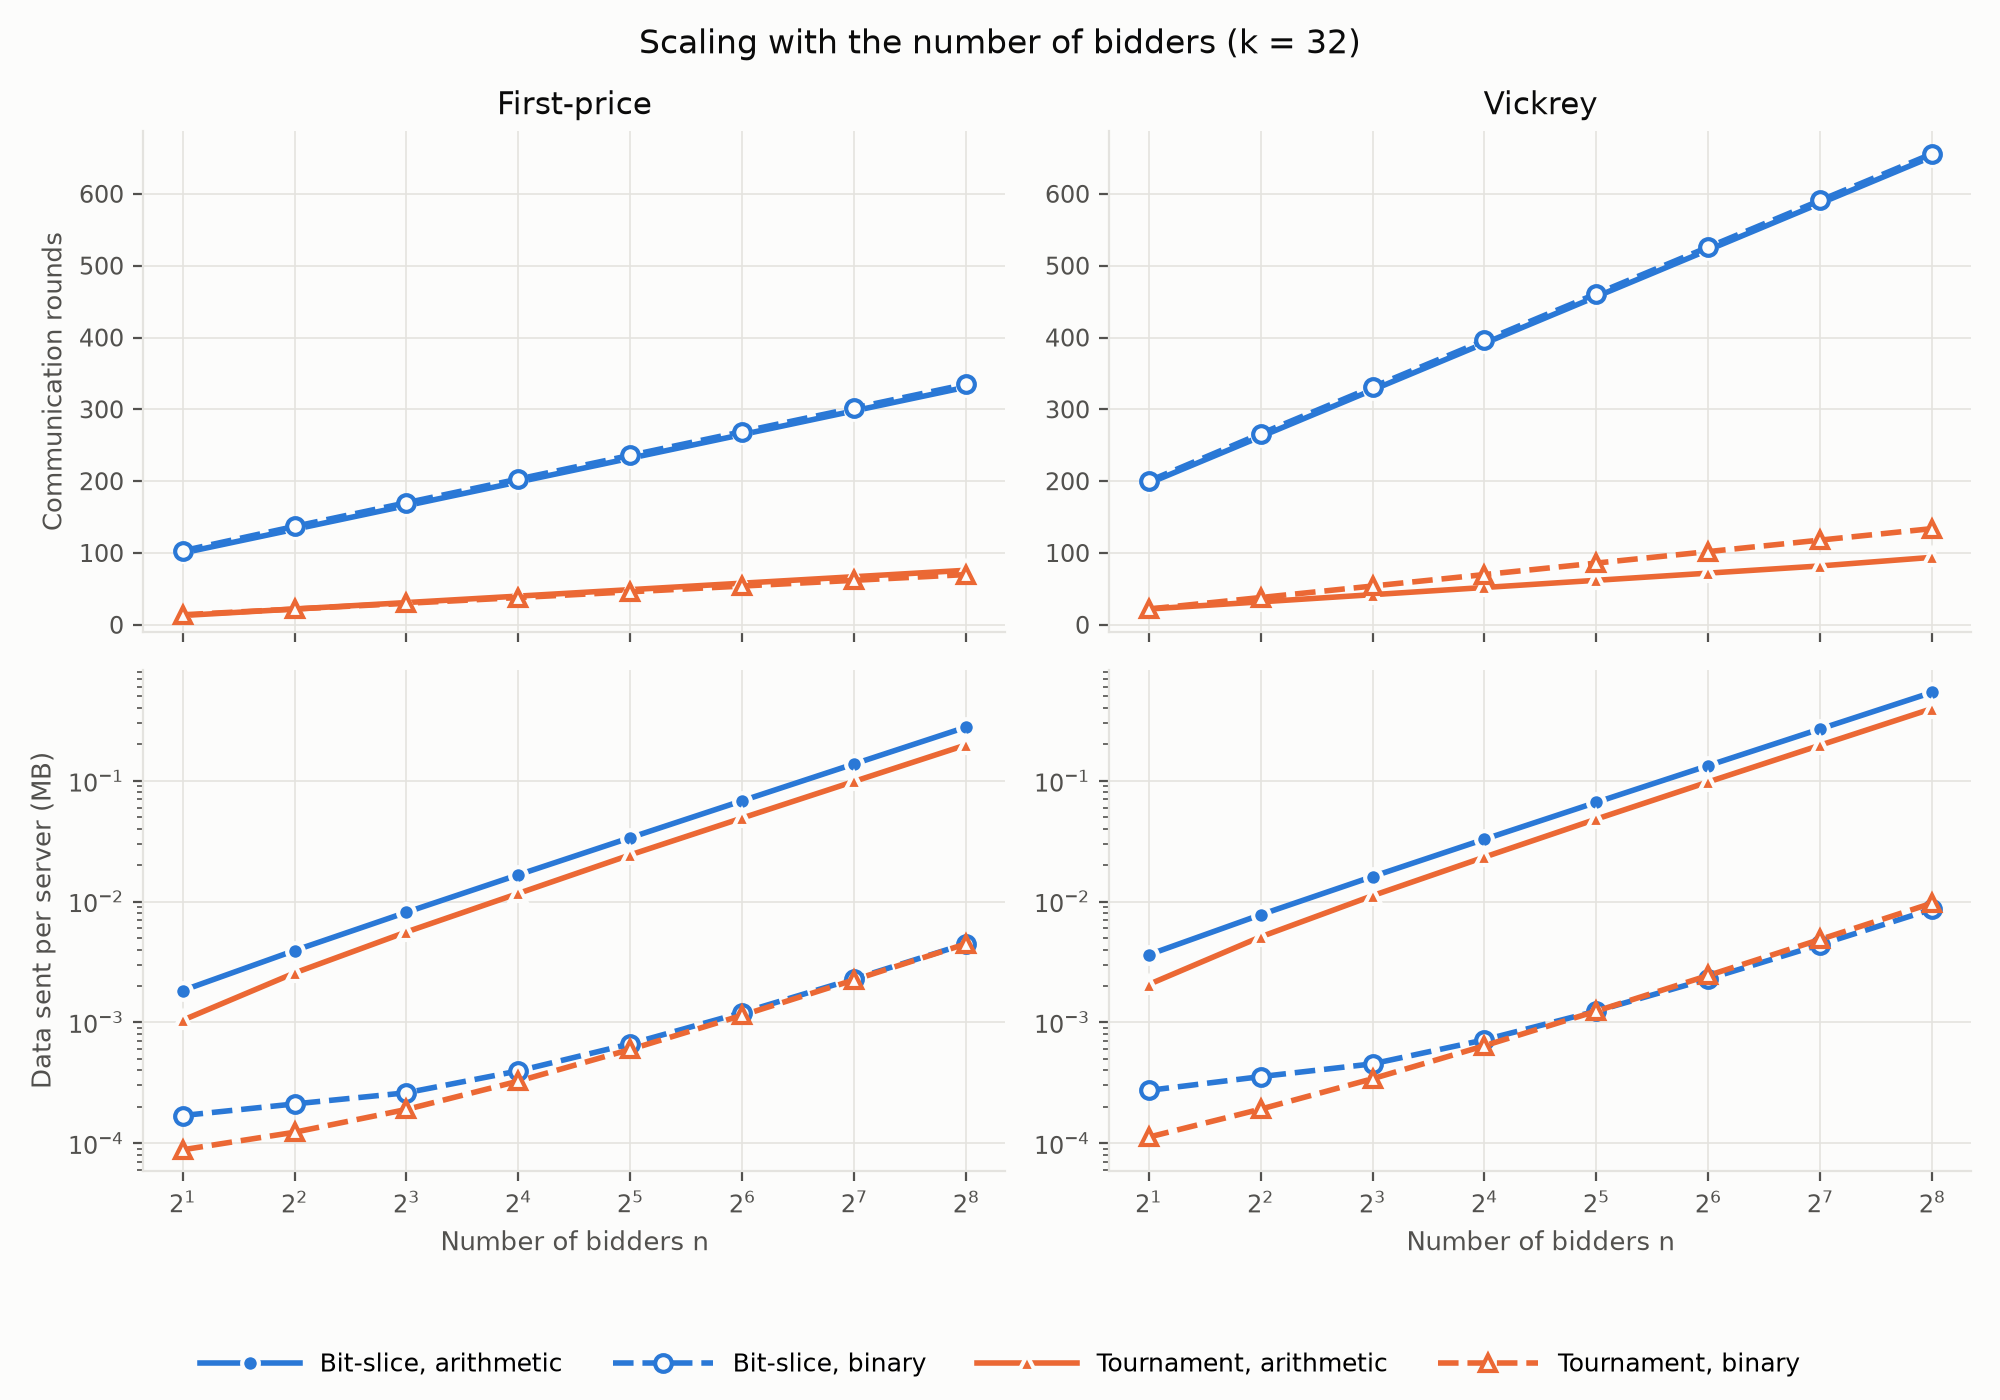
\includegraphics[height=0.78\textheight]{../bench/results/fig_scale_n.png}\\[2pt]
  \footnotesize 3 servers on one machine. The measured AND counts match our formula exactly.
\end{frame}

\begin{frame}{Results at $n = 128$, $k = 32$, Vickrey}
  \small
  \begin{tabular}{@{}lrrrrr@{}}
    \toprule
    Variant & ANDs & rounds & MB / server & LAN (s) & WAN (s) \\
    \midrule
    Bit-slice, arithmetic  & 29\,505 & 587 & 0.269  & 0.61 & 29.4 \\
    Bit-slice, binary      & 29\,505 & 591 & \textbf{0.0044} & 0.61 & 29.6 \\
    Tournament, arithmetic & 15\,621 & \textbf{82} & 0.197 & \textbf{0.09} & \textbf{4.1} \\
    Tournament, binary     & 34\,163 & 118 & 0.0049 & 0.12 & 5.9 \\
    \bottomrule
  \end{tabular}
  \medskip

  \begin{columns}[T]
    \begin{column}{0.48\textwidth}
      \begin{exampleblock}{Binary domain: $61\times$ less data}
        each AND costs 1 bit instead of 64.
        The baseline gains just as much.
      \end{exampleblock}
    \end{column}
    \begin{column}{0.48\textwidth}
      \begin{alertblock}{But rounds decide the time}
        bit-slice handles bits one after another: rounds grow with $k \log n$.
        The tournament needs far fewer.
      \end{alertblock}
    \end{column}
  \end{columns}
  \footnotesize LAN: 1 ms, 1 Gbit/s. WAN: 50 ms, 100 Mbit/s. Modelled from measured rounds and bytes.
\end{frame}

\begin{frame}{Modelled network time and the cost of malicious security}
  \begin{columns}[c]
    \begin{column}{0.54\textwidth}
      \centering
      \fig{fig_wan.png}
    \end{column}
    \begin{column}{0.44\textwidth}
      \centering
      \fig{fig_security.png}
    \end{column}
  \end{columns}
  \medskip

  \small Same programs under malicious-security protocols: $\approx 6\times$ data in the arithmetic domain;
  near-constant $\approx$0.11 MB in the binary domain.
\end{frame}

\begin{frame}{How we checked correctness}
  Every result is compared with the \textbf{plain, non-private auction rule}.
  \begin{itemize}
    \item \textbf{The formulas:} simulated on plain bits for every input with up to 3 bidders,
          plus thousands of random cases with forced ties
    \item \textbf{The real protocol:} three servers run edge cases (ties, one bidder, all zero,
          maximum bids) and random auctions, also under malicious security
    \item \textbf{The output:} only the winner and the price are opened
    \item \textbf{The benchmarks:} every run's result checked as well
  \end{itemize}
\end{frame}

\begin{frame}{What we learned}
  \begin{itemize}
    \item \textbf{The domain matters more than the algorithm.}
          Binary vs.\ arithmetic: $61\times$ communication; bit-slice vs.\ tournament: about 10\%.
    \item \textbf{Bit-slice loses on latency.} Its scan is sequential in the bid length; modern
          comparisons need only $O(\log k)$ rounds. Kurosawa--Ogata's ``$7\times$ faster'' was
          measured against 2002-era comparisons.
    \item \textbf{Where bit-slice still wins:} fewest ANDs at large $n$ (binary), exactly 2
          opened values, only multiplication needed, and it ports to server-free designs (SEAL).
    \item \textbf{Secret data forces branch-free algorithms.} Every ``if'' on a secret becomes
          arithmetic, so the same operations run whatever the bids are.
  \end{itemize}
\end{frame}

\begin{frame}{Limitations and future work}
  \begin{columns}[T]
    \begin{column}{0.48\textwidth}
      \textbf{Limitations}
      \begin{itemize}
        \item bidders are trusted to send valid bits
        \item a malicious server could swap its own input share
        \item all servers on one machine; network times modelled
      \end{itemize}
    \end{column}
    \begin{column}{0.48\textwidth}
      \textbf{Future work}
      \begin{itemize}
        \item authenticated bidder inputs
        \item public verifiability: commitments + ZK proofs
        \item radix-$2^r$ scan: $r\times$ fewer rounds
        \item more servers (Shamir); SEAL (no servers)
      \end{itemize}
    \end{column}
  \end{columns}
  \bigskip
  \begin{exampleblock}{Summary}
    Three servers compute a first-price or Vickrey auction without any of them seeing a bid,
    and open only the winner and the price.
  \end{exampleblock}
\end{frame}

\begin{frame}[standout]
  Thank you!\\[10pt]
  \normalsize Questions?\\[14pt]
  \footnotesize \texttt{github.com/rcharan05/CS670\_Project}
\end{frame}

\end{document}
